\chapter{Моделирование модуля активного управления
  трафиком сети передачи данных}

\section{Создание модуля для среды Mininet}

В главе 2 уже был рассмотрен способ моделирования сети в среде
Mininet.  Данный способ включает в себя создание программы на языке
программирования Python. В программе описывается топология сети,
манипуляции с сетью, ее старт и завершение. Написав пару таких сетей,
можно столкнуться с мыслью, что части кода идентичны друг другу, а
каждое редактирование и исследование сети занимает время. Можно
написать автоматизированное решение, которое требует только задание
нужных сетевых элементов и их конфигураций, а программа сама считает
данные, создаст сеть, построит графики сетевых характеристик и
т.\,д. Данная идея будет описана далее в этой главе.

Для начала требуется выбрать формат конфигурационного файла. Выбор
формата конфигурационного файла производится из собственных
предпочтений и удобства анализа файла. В данной работе будет
использован формат toml~\cite{toml}.

Определим объекты сети, которые мы будем описывать в конфигурационном
файле: хосты, коммутаторы, соединения, мониторинговые характеристики,
команды qdisc для интерфейсов коммутатора.  Имея подобный
конфигурационный toml-файл, его можно прочесть с помощью средств
Python, обработать и положить требуемые значения в объекты.  Такой
подход позволяет строить сколь угодно большие топологии без правки
логики приложения. На основе данного файла можно построить программу,
использующую диаграмму активностей, показанную на рис.~\ref{fig:30001}.

\begin{figure}[!h]
  \centering 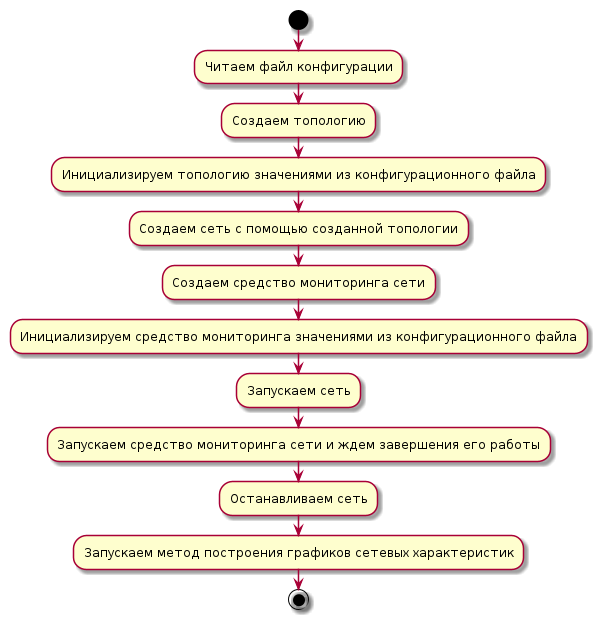
\includegraphics[width=0.7\textwidth]{image/act_dia.png}
  \caption{Диаграмма активностей приложения}
  \label{fig:30001}
\end{figure}

Программу можно разделить на такие модули как: мониторинг сети,
построение графиков сетевых характеристик, модуль модели сети, который
включает в себя топологию сети и два предыдущих элемента. Исходя из
этого можно построить диаграмму классов приложения, показанную на
рис.~\ref{fig:30002}.

\begin{figure}[!h]
\centering
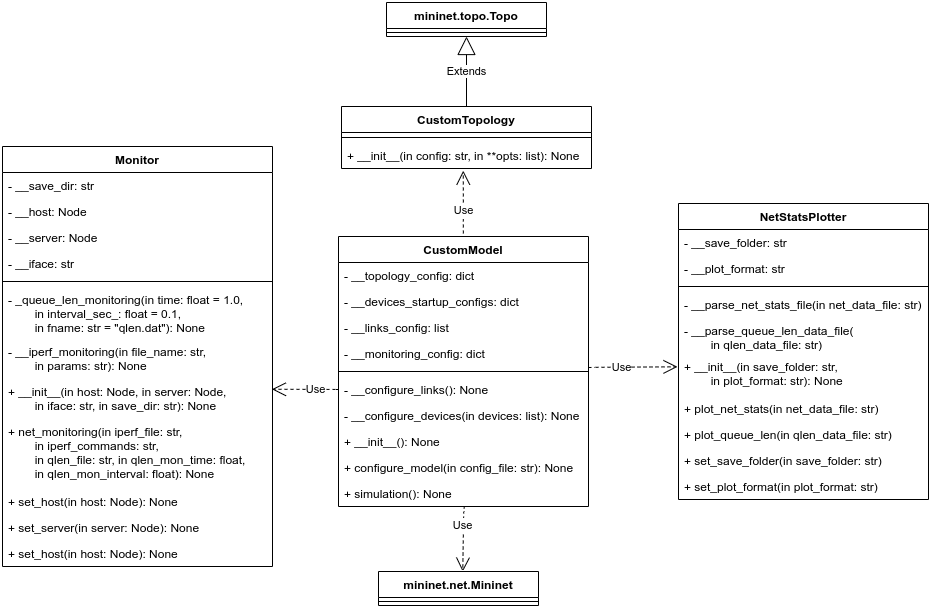
\includegraphics[width=0.9\textwidth]{image/class_dia.png}
\caption{Диаграмма классов приложения}
\label{fig:30002}
\end{figure}

Главным классом, включающим в себя все остальные, является
CustomModel.  В методе simulation создаются объекты классов Monitor,
mininet.net.Mininet, CustomTopology и NetStatsPlotter.

Рассмотрим подробнее классы, создаваемые в методе simulation:
\begin{itemize}
\item mininet.net.Minet --- предоставляемый Mininet API класс,
  отвечающий за создание сети с топологией, указанной в
  CustomTopology;
\item CustomTopology --- класс топологии сети;
\item Monitor --- класс, в котором происходят замеры сетевых
  характеристик исследуемой сети;
\item NetStatsPlotter --- класс, объект которого занимается
  построением графиков сетевых характеристик.
\end{itemize}

Код классов NetStatsPlotter, Monitor, CustomTopology и CustomModel
находятся в приложениях A, B, C, D
% \protect\hyperlink{appendix1}
%{приложении A}, 
% \protect\hyperlink{appendix2}
%{приложении B}, 
%\protect\hyperlink{appendix3}
%{приложении C} и 
%\protect\hyperlink{appendix4}
%{приложении D}
соответственно.

Точкой входа в данную программу будет файл main.py. Содержимое данного
файла представлено ниже:

\begin{minted}[breaklines,frame=lines,linenos,framesep=2mm,baselinestretch=1.2,fontsize=\footnotesize]{python}
#!/usr/bin/python3.8

import argparse
from model.CustomModel import CustomModel

if __name__ == '__main__':
    parser = argparse.ArgumentParser()
    h = "Файл конфигурации"
    parser.add_argument('-c', '--config', type=str, help=h)
    args = parser.parse_args()
    if args.config:
        top = CustomModel()
        top.configure_model(args.config)
        top.simulation()
    else:
        print("Введите название конфиг-файла")

\end{minted}

Это обычный скрипт на языке программирования Python, который создает
модель нашей сети из конфигурационного файла, переданного параметром
командной строки. Запустить данный скрипт можно с помощью команды
\begin{minted}[breaklines]{bash}
  sudo ./main.py -c config/pfifo_config.toml
\end{minted}

Параметр \textbf{-c} отвечает за местоположение конфигурационного
файла.  Естественно, перед запуском скрипта требуется задать право на
исполнение файла. Делается это с помощью команды
\begin{minted}[breaklines]{bash}
  chmod +x main.py
\end{minted}

После запуска программы в каталоге приложения появится директория с
именем, которое было указано в toml-файле. В ней содержатся графики
изменения сетевых характеристик и сырые данные, которые были
обработаны объектом класса NetStatsPlotter.

\section{Тестирование программного модуля}

У нас имеется готовая программа в наличии и нам следует ее
протестировать. Для начала требуется описать сеть, заполнить
конфигурационный файл по характеристикам заданной сети, запустить
программу и исследовать сетевые характеристики сети передачи данных.

Пусть у нас имеется сеть, заданная топологией, приведенной на
рис.~\ref{fig:30003}.

\begin{figure}[!h]
\centering
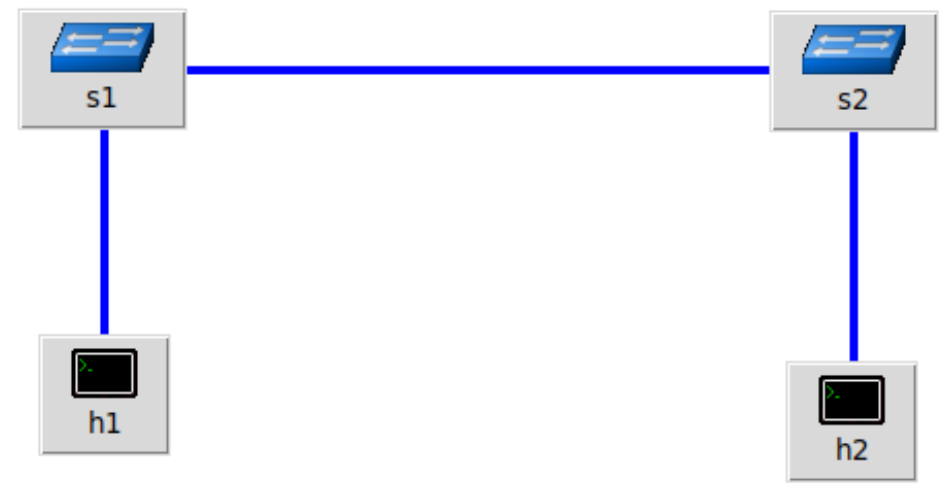
\includegraphics[width=0.5\textwidth]{image/example_topo.png}
\caption{Топология исследуемой сети}
\label{fig:30003}
\end{figure}

Предполагается, что в данной сети будут действовать следующие правила:
\begin{itemize}
\item скорость передачи данных ограничена;
\item максимальная пропускная способность соединения h1-s1 равна 100
  Мбит/с;
\item максимальная пропускная способность соединения s2-h2 равна 50
  Мбит/с;
\item на коммутаторе s2 стоит дисциплина обработки очередей FIFO с
  максимальным количеством пакетов, равным 60;
\item потери в сети составляют 0.001\%;
\item задержка имеет нормальное распределение с математическим
  ожиданием в 30 мс и с дисперсией в 7 мс.
\item в сети работает алгоритм для работы с перегрузками TCP Reno.
\end{itemize}

Опишем данные характеристики в конфигурационном файле.
\begin{minted}[breaklines,frame=lines,linenos,framesep=2mm,baselinestretch=1.2,fontsize=\footnotesize]{python}
# device settings
[devices]
    [devices.h1]
        name = "h1"
        ip = "10.0.0.1"
        cmd = [ "sysctl -w net.ipv4.tcp_congestion_control=reno" ]
    [devices.h2]
        name = "h2"
        ip = "10.0.0.2"
        cmd = [ "sysctl -w net.ipv4.tcp_congestion_control=reno" ]

# switch settings
[switches]
    [switches.s1]
        name = "s1"
    [switches.s2]
        name = "s2"

# link settings
[links]
pairs = [
    ["h1", "s1"],
    ["s1", "s2"],
    ["s2", "h2"]
]
cmd = [
    "tc qdisc replace dev s1-eth2 root handle 10: tbf rate 100mbit burst 50000 limit 150000",
    "tc qdisc add dev s1-eth2 parent 10: handle 20: netem loss 0.001% delay 30ms 7ms distribution normal",
    "tc qdisc replace dev s1-eth1 root handle 10: tbf rate 100mbit burst 50000 limit 150000",
    "tc qdisc add dev s1-eth1 parent 10: handle 20: netem loss 0.001% delay 30ms 7ms distribution normal",
    "tc qdisc replace dev s2-eth2 root handle 10: tbf rate 50mbit burst 25000 limit 75000",
    "tc qdisc add dev s2-eth2 parent 10: handle 15: pfifo limit 30",
    "tc qdisc replace dev s2-eth1 root handle 10: tbf rate 50mbit burst 25000 limit 75000"
]

[monitoring]
monitoring_time = 60
monitoring_interval = 0.005
host_client = "h1"
host_server = "h2"
interface = "s2-eth2"
iperf_file_name = "iperf.json"
iperf_flags = ""
queue_data_file_name = "qlen.data"
plots_dir = "plots_dir_first"
\end{minted}

В представленном toml-файле раздел \textbf{devices} отвечает за
настройку конечных узлов сети, раздел \textbf{switches} отвечает за
настройку коммутаторов, а раздел \textbf{links} отвечает за настройку
соединений узлов сети и конфигурацию интерфейсов коммутаторов.

На хостах указывается ip-адрес, имя хоста и алгоритм работы с
перегрузками. На коммутаторах прописывается только имя, однако, список
настроек можно расширить, изменив программную логику в классе с
топологией. В разделе \textbf{links} явно указывается, какие пары
сетевых устройств соединяются, и команды, которые настраивают дисциплину
очередей на интерфейсах. Важно уточнить, что соединения на коммутаторе
происходят последовательно, т.\,е. если первым идет подключение h1-s1, то
интерфейсом на коммутаторе, отвечающим за данное соединение, является
интерфейс s1-eth1. Если, например, подключить еще одно устройство к
коммутатору, то интерфейсом коммутатора в соединении будет s1-eth2, и
так далее. Данный момент следует учитывать при установке правил
дисциплин очередей на интерфейсах.

Также, в toml-файле имеется блок \textbf{monitoring}, в котором заданы
следующие параметры:
\begin{itemize}
\item monitoring\_time --- время мониторинга сети в секундах;
\item monitoring\_interval --- интервалы между замерами длины очереди
  в секундах;
\item host\_client --- узел, который будет отправлять данные;
\item host\_server --- узел, который будет принимать данные;
\item interface --- интерфейс, на котором будет мониторится размер
  очереди;
\item iperf\_file\_name --- имя файла с отчетом мониторинга iperf;
\item iperf\_flags --- iperf-флаги клиента;
\item queue\_data\_file\_name --- имя файла с отчетом мониторинга
  длины очереди;
\item plots\_dir --- директория со всеми графиками сетевых
  характеристик.
\end{itemize}

Все параметры являются обязательными.

Запуск программы показан рис. \ref{fig:30004}.

\begin{figure}[H]
  \centering
  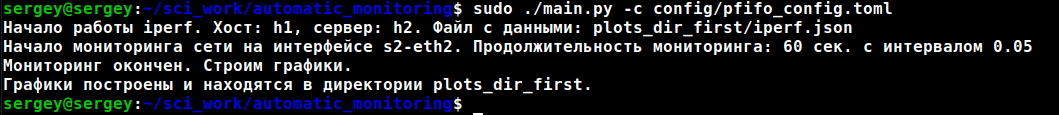
\includegraphics[width=1.0\textwidth]{image/ch03_01/prog_start1.png}
  \caption{Запуск программы}
  \label{fig:30004}
\end{figure}

Рассмотрим получившиеся графики сетевых характеристик:
\begin{itemize}
\item На рис. \ref{fig:30005} приведен график, показывающий динамику
  объема переданных.

  \begin{figure}[H]
  \centering
  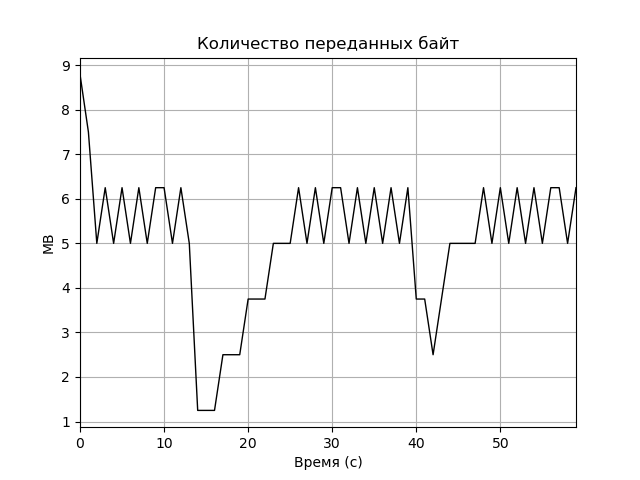
\includegraphics[width=0.55\textwidth]{image/ch03_01/bytes.png}
\caption{График изменения количества переданных данных с течением
  времени}
\label{fig:30005}
\end{figure}

\item На рис. \ref{fig:30006} приведен график изменения значений окна
  перегрузки TCP Reno.

\begin{figure}[H]
\centering
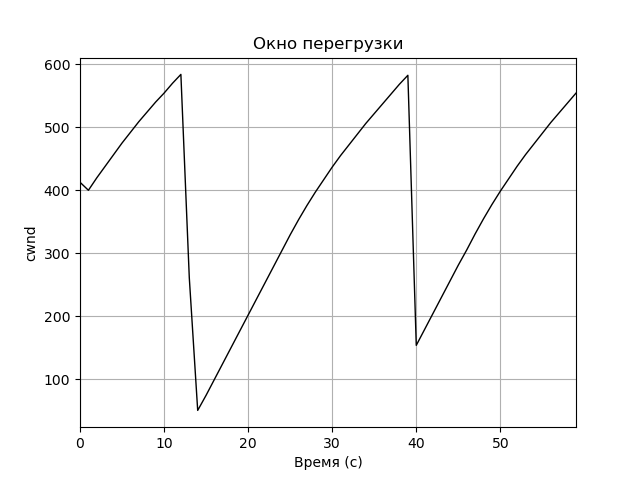
\includegraphics[width=0.55\textwidth]{image/ch03_01/cwnd.png}
\caption{График изменения значения окна перегрузки с течением времени
  при использовании алгоритма TCP Reno}\label{fig:30006}
\end{figure}


\item Динамика значений RTT (измеряется в миллисекундах)
  демонстрируется на рис.~\ref{fig:30007}.

\begin{figure}[H]
\centering
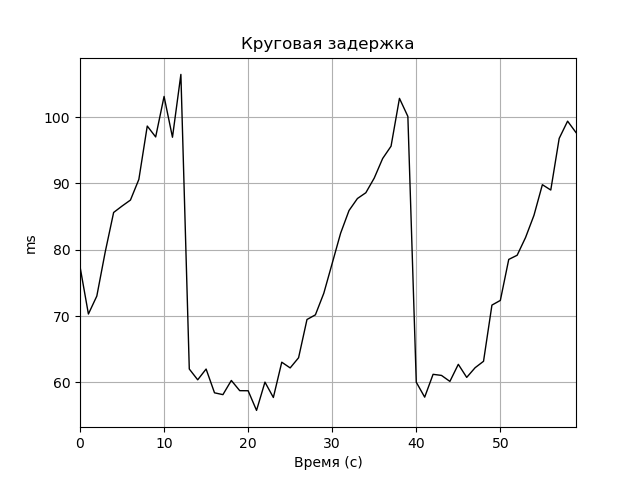
\includegraphics[width=0.65\textwidth]{image/ch03_01/rtt.png}
\caption{График изменения значения RTT с течением
времени}\label{fig:30007}
\end{figure}


\item График отклонений значений RTT приведен на рис.~\ref{fig:30008}.

\begin{figure}[H]
\centering
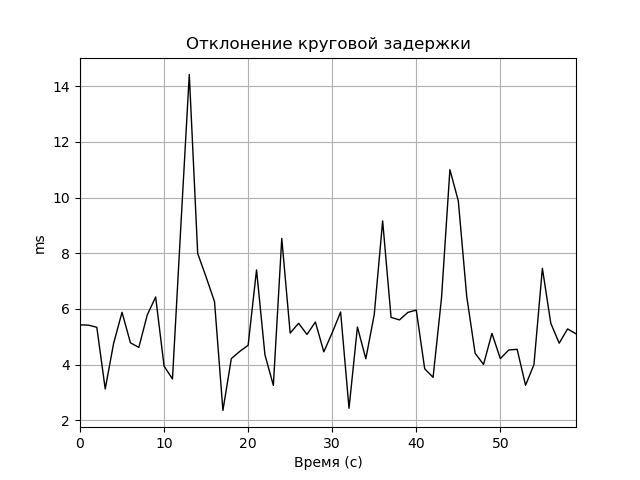
\includegraphics[width=0.65\textwidth]{image/ch03_01/rttvar.png}
\caption{График изменения значения вариации RTT с течением времени}
\label{fig:30008}
\end{figure}

\item Динамика изменения пропускной способности показана на
  рис.~\ref{fig:30009}.

  \begin{figure}[H]
\centering
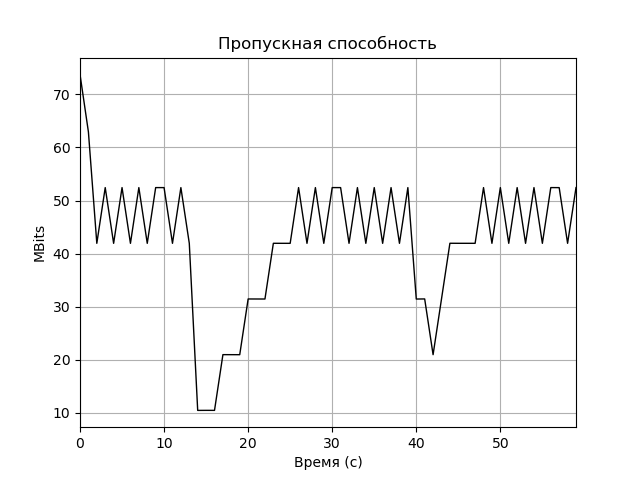
\includegraphics[width=0.65\textwidth]{image/ch03_01/throughput.png}
\caption{График изменения значения пропускной способности с течением
  времени}
\label{fig:30009}
\end{figure}

\item Изменение длины очереди на интерфейсе s2-eth2 показано на
  рис.~\ref{fig:30010}.

\begin{figure}[H]
\centering
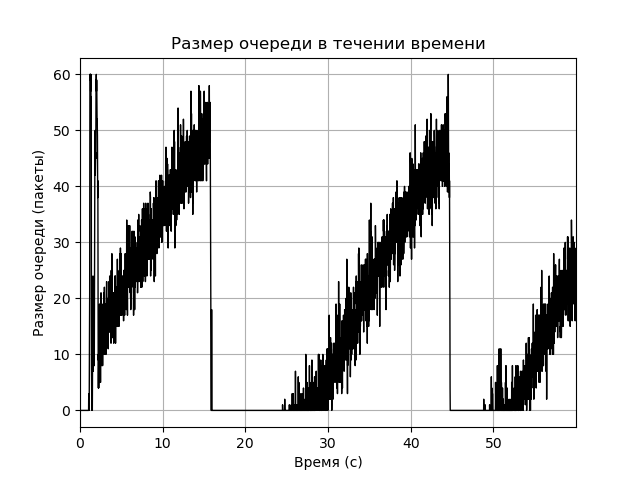
\includegraphics[width=0.65\textwidth]{image/ch03_01/queue_len.png}
\caption{График изменения длины очереди на интерфейсе
  s2-eth2}
\label{fig:30010}
\end{figure}

\item Изменение значения количества повторно переданных пакетов
  показано на рис.~\ref{fig:30011}.

\begin{figure}[H]
  \centering
  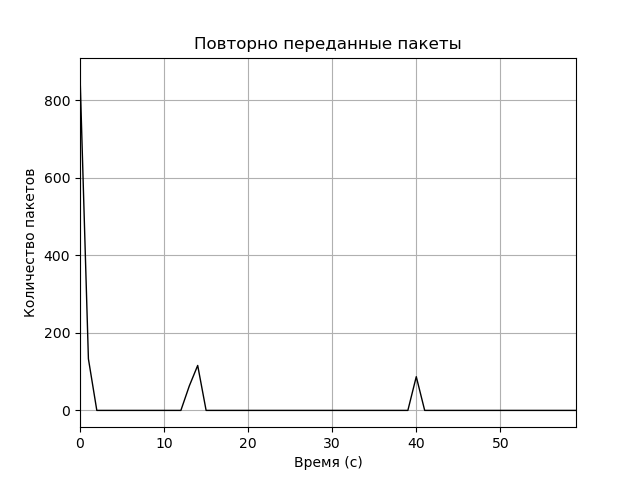
\includegraphics[width=0.65\textwidth]{image/ch03_01/retransmits.png}
\caption{График изменения значения повторно переданных пакетов во
  времени}
\label{fig:30011}
\end{figure}

\end{itemize}







Из графиков четко видно, что пропускная способность заметно снижается,
когда размер окна уменьшается. График CWND показывает, что таких
уменьшений размера окна 3 и связаны они с потерей пакетов. Потери в
сети обусловлены ненадежностью линии передачи данных и размером длины
очереди на интерфейсе коммутатора. Так как при моделировании выбирался
самый простой тип дисциплины очередей droptail (pfifo), то на графике
изменения длины очереди можно увидеть, что пакеты начинают
сбрасываться при достижении критического значения длины очереди (в
нашем случае 60 пакетов).  При увеличении длины
очереди пакеты достигают получателя медленнее и значение RTT растет
пропорционально увеличению размера очереди.

\section{Пример простой сети с несколькими хостами}

Сеть, в которой существуют только хост-сервер и хост-клиент встречаются
довольно редко. Требуется усложнить модель сети, добавив в нее несколько
хостов, которые в некоторый промежуток времени начинают передавать
данные на сервер. Реализовать временные задержки довольно легко, если
вспомнить про существование скриптовых файлов, которые можно запустить
на хостах. Внутри данного файла будет настройка хоста, подключение к
серверу и симуляция задержек во времени с помощью утилиты sleep~\cite{sleep}.

Пусть у нас имеется сеть, заданная топологией, приведенной на
рис.~\ref{fig:30012}.

\begin{figure}[!h]
\centering
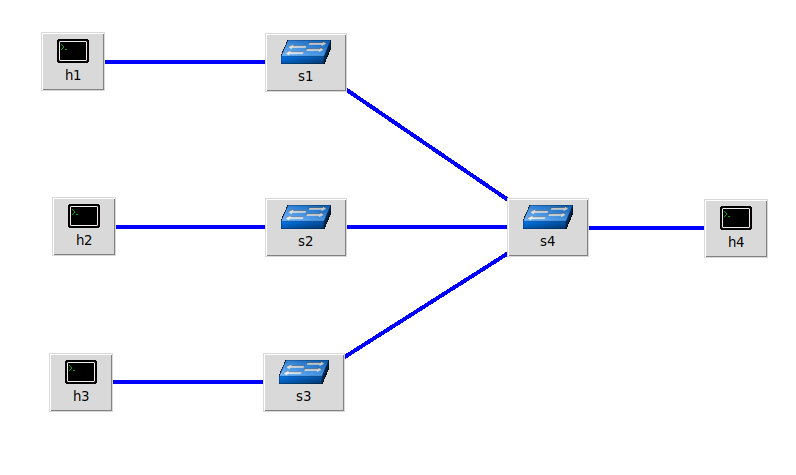
\includegraphics[width=0.7\textwidth]{image/ch03_02/example_topo.png}
\caption{Топология исследуемой сети}
\label{fig:30012}
\end{figure}

Предполагается, что в данной сети будут действовать следующие правила:
\begin{itemize}
\item скорость передачи данных ограничена;
\item максимальная пропускная способность соединения s4-s1 равна 15
  Мбит/с;
\item максимальная пропускная способность соединения s4-s2 равна 10
  Мбит/с;
\item максимальная пропускная способность соединений s4-s3 и s4-h4
  равна 20 Мбит/с;
  % \item максимальная пропускная способность соединения s4-h4 равна
  %   20 Мбит/с;
\item на коммутаторе s4 стоит дисциплина обработки очередей FIFO с
  максимальным количеством пакетов, равным 45;
\item потери в сети составляют 0.001\%;
\item задержка имеет нормальное распределение с математическим
  ожиданием в 10 мс и с дисперсией в 3 мс.
\item в сети работает алгоритм для работы с перегрузками TCP BBR.
\end{itemize}

Предполагается, что h2 начнет передавать данные на сервер через 10
секунд после старта сети и время передачи равняется 20 секундам, а h3
начнет передавать данные через 20 секунд с таким же временем передачи. В
данной сети коммутаторы s1, s2, s3 существуют лишь для технической
реализации сетевых задержек, потерь и ограничения скорости передачи
данных.

Опишем данные характеристики в конфигурационном файле.
\begin{minted}[breaklines,frame=lines,linenos,framesep=2mm,baselinestretch=1.2,fontsize=\footnotesize]{python}
# device settings
[devices]
    [devices.h1]
        name = "h1"
        ip = "10.0.0.1"
        cmd = [ "sysctl -w net.ipv4.tcp_congestion_control=bbr" ]
    [devices.h2]
        name = "h2"
        ip = "10.0.0.2"
        cmd = [ "./config/host_configs/h2.sh" ]
    [devices.h3]
        name = "h3"
        ip = "10.0.0.3"
        cmd = [ "./config/host_configs/h3.sh" ]
    [devices.h4]
        name = "h4"
        ip = "10.0.0.4"
        cmd = [
            "iperf3 -s -p 7778 -1",
            "iperf3 -s -p 7779 -1",
        ]
# switch settings
[switches]
    [switches.s1]
        name = "s1"
    [switches.s2]
        name = "s2"
    [switches.s3]
        name = "s3"
    [switches.s4]
        name = "s4"
# link settings
[links]
pairs = [
    ["h1", "s1"],
    ["h2", "s2"],
    ["h3", "s3"],
    ["s1", "s4"],
    ["s2", "s4"],
    ["s3", "s4"],
    ["s4", "h4"]
]
cmd = [
    "tc qdisc replace dev s4-eth4 root handle 10: tbf rate 20mbit burst 10000 limit 30000",
    "tc qdisc replace dev s4-eth1 root handle 10: tbf rate 20mbit burst 10000 limit 30000",
    "tc qdisc replace dev s4-eth2 root handle 10: tbf rate 20mbit burst 10000 limit 30000",
    "tc qdisc replace dev s4-eth3 root handle 10: tbf rate 20mbit burst 10000 limit 30000",
    "tc qdisc add dev s4-eth4 parent 10: handle 15: pfifo limit 45",
    "tc qdisc replace dev s1-eth2 root handle 10: tbf rate 15mbit burst 7500 limit 22500",
    "tc qdisc replace dev s2-eth2 root handle 10: tbf rate 10mbit burst 5000 limit 15000",
    "tc qdisc replace dev s3-eth2 root handle 10: tbf rate 20mbit burst 10000 limit 30000",
    "tc qdisc replace dev s1-eth1 root handle 10: tbf rate 15mbit burst 7500 limit 22500",
    "tc qdisc replace dev s2-eth1 root handle 10: tbf rate 10mbit burst 5000 limit 15000",
    "tc qdisc replace dev s3-eth1 root handle 10: tbf rate 20mbit burst 10000 limit 30000",
    "tc qdisc add dev s1-eth2 parent 10: handle 20: netem loss 0.001% delay 10ms 3ms distribution normal",
    "tc qdisc add dev s2-eth2 parent 10: handle 20: netem loss 0.001% delay 10ms 3ms distribution normal",
    "tc qdisc add dev s3-eth2 parent 10: handle 20: netem loss 0.001% delay 10ms 3ms distribution normal",
    "tc qdisc add dev s1-eth1 parent 10: handle 20: netem loss 0.001% delay 10ms 3ms distribution normal",
    "tc qdisc add dev s2-eth1 parent 10: handle 20: netem loss 0.001% delay 10ms 3ms distribution normal",
    "tc qdisc add dev s3-eth1 parent 10: handle 20: netem loss 0.001% delay 10ms 3ms distribution normal"
]
[monitoring]
monitoring_time = 60
monitoring_interval = 0.05
host_client = "h1"
host_server = "h4"
interface = "s4-eth4"
iperf_file_name = "iperf.json"
iperf_flags = "-b 15mbit"
queue_data_file_name = "qlen.data"
plots_dir = "plots_dir_second"
\end{minted}

Видно, что здесь, в разделе настроек хостов, у хоста h4 запускаются 2
iperf-сервера. К ним через скрипт-файлы подключатся хосты h2 и h3.

Скрипт-файл для хоста h2:
\begin{minted}{bash}
#!/bin/bash
sysctl -w net.ipv4.tcp_congestion_control=bbr
sleep 10
iperf3 -c 10.0.0.4 -p 7778 -t 20
\end{minted}

Скрипт-файл для хоста h3:
\begin{minted}{bash}
#!/bin/bash
sysctl -w net.ipv4.tcp_congestion_control=bbr
sleep 20
iperf3 -c 10.0.0.4 -p 7779 -t 20
\end{minted}

Запустим данную сеть и рассмотрим наиболее интересующие нас графики
сетевых характеристик.

Динамика изменения пропускной способности показана на
рис.~\ref{fig:30015}. Видно, что наименьшее значение пропускной
способности достигалось в промежутке, когда одновременно все хосты
передавали данные на сервер. Помимо этого, на графике четко видно
сколько хостов ведут передачу данных.

\begin{figure}[!h]
\centering
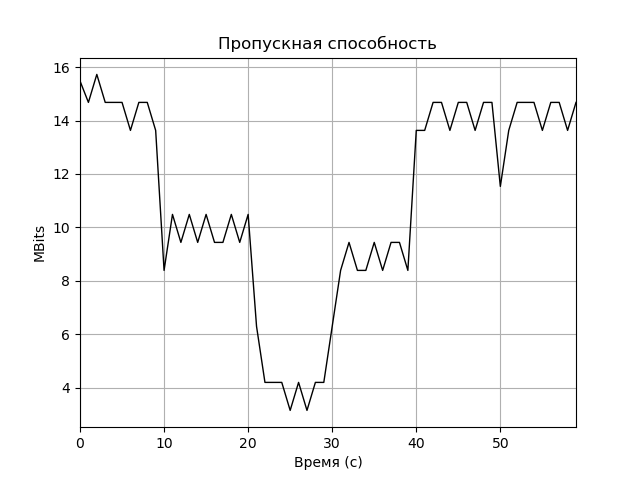
\includegraphics[width=0.55\textwidth]{image/ch03_02/throughput.png}
\caption{График изменения значения пропускной способности с течением
времени}\label{fig:30015}
\end{figure}

На рис. \ref{fig:30013} приведен график изменения значений окна
перегрузки TCP BBR (CWND). %На графике видно, что
Наибольшее значение CWND достигается, % только тогда
когда 1 хост передает данные на сервер, а все остальные молчат.

\begin{figure}[!h]
\centering
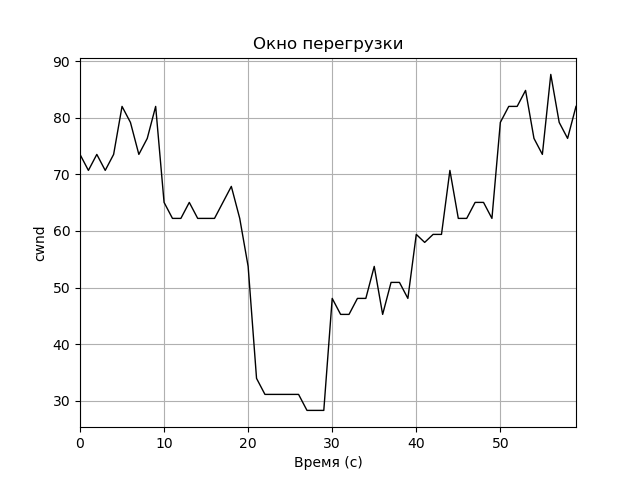
\includegraphics[width=0.55\textwidth]{image/ch03_02/cwnd.png}
\caption{График изменения значения окна перегрузки с течением времени
% при использовании алгоритма
(TCP Reno)}\label{fig:30013}
\end{figure}

Динамика значений RTT демонстрируется на рис.~\ref{fig:30014}~--- %. Видно,
RTT увеличивается пропорционально росту окна перегрузки.

\begin{figure}[!h]
\centering
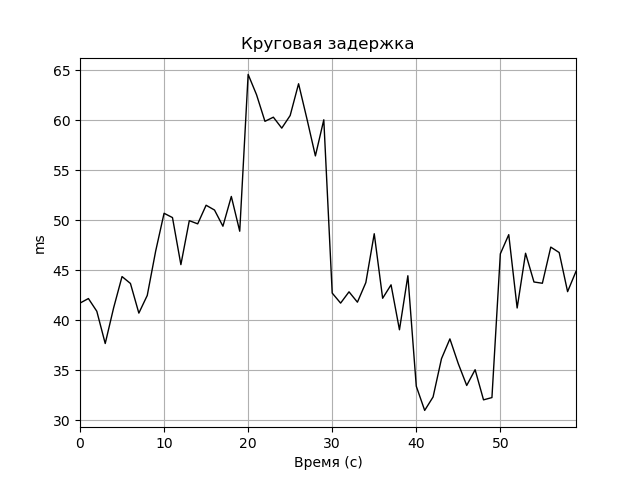
\includegraphics[width=0.52\textwidth]{image/ch03_02/rtt.png}
\caption{График изменения значения RTT с течением
  времени}\label{fig:30014}
\end{figure}

% \vfill

